\subsection{Einführung}
\label{subsec:voronoi-introduction}

Gegeben seien gem.~\cite{klein2005algorithmischegeometrie} und~\cite{atsuyuki2000spatialtessellations} die folgenden Probleme:

\begin{compactitem}
\item ein Astronom, der die Struktur des Universum studiert
\item ein Archäologe, der die Regionen verschiedener neolithischer Klans untersucht
\item ein Meteorologe, der versucht den Niederschlag von einem defekten Messgerät abzuschätzen
\item ein Städte-Planer, der versucht öffentliche Schulen in einer Stadt zu lokalisieren
\item ein Tourist, der die nächste Poststelle sucht
\item die Bestimmung der nächsten Nachbarn
\item die Bestimmung des minimalen Spannbaumes
\item die Bestimmung des grössten leeren Kreises
\end{compactitem}

\noindent\hspace*{0mm} \\Sie fragen sich nun bestimmt, was diese Probleme gemeinsam haben. Auf den ersten Blick haben sie nichts gemeinsam. Obige Probleme können jedoch mit Ansätzen, welche aus einem einzelnen Konzept entwickelt wurden, gelöst werden: \textbf{Voronoi-Diagrammen} (\citeyear{atsuyuki2000spatialtessellations}, S. 1).

1644 äusserte Descartes in seinem Buch über die Prinzipien der Philosophie die Vermutung, dass das Sonnensystem aus Materie besteht, welche um Fixsterne herumwirbelt.
Auch wenn die Theorie so nicht richtig ist, enthält sie das grundlegende Prinzip der Voronoi-Diagramme~\parencite[S. 209]{klein2005algorithmischegeometrie}.

Gegeben sei ein \textit{m}-dimensionaler Raum $\mathbb{R}^m$ und in diesem eine Menge $O = {p, q, r, s \dots}$ von Objekten bzw. Punkten, die auf ihre Umgebung einen Einfluss ausüben. Hier kann man folgende Zerlegung des Raumes in Regionen betrachten: Zu jedem Objekt $p$ in $O$ bildet man die (Voronoi-) Region $VR(p, O)$. Diese beinhaltet nun alle Punkte, für die der von $p$ ausgeübte Einfluss am stärksten ist~\parencite[S. 209]{klein2005algorithmischegeometrie}.
\newpage{}

\begin{figure}[h]
\centering
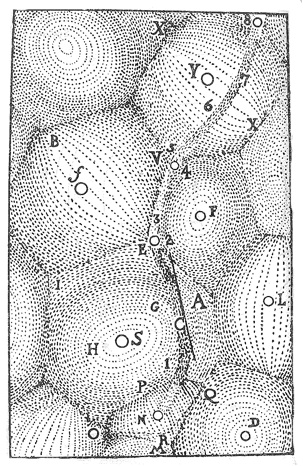
\includegraphics[width=150px]{images/descartes_vortices.jpg}
\caption{Wirbelkammern gem. Descartes\protect\footnotemark}
\label{fig:descartesVortices}
\end{figure}
\footnotetext{\cite{slowik2013}}

Um auf das Beispiel von Descartes zurückzukommen: Durch die Anziehungskraft von Fixsternen (in Abbildung~\ref{fig:descartesVortices} sind dies z.B. $\mathnormal{f}$, $F$ oder $Y$) entstehen Wirbel \parencite[S. 209]{klein2005algorithmischegeometrie}.
